\documentclass[12pt, a4paper]{article} % book, report, article, letter, slides
                                       % letterpaper/a4paper, 10pt/11pt/12pt, twocolumn/twoside/landscape/draft

%%%%%%%%%%%%%%%% PACKAGES %%%%%%%%%%%%%%%%%%%%%

\usepackage[utf8]{inputenc} % encoding

\usepackage[english]{babel} % use special characters and also translates some elements within the document.

\usepackage{amsmath}        % Math
\usepackage{amsthm}         % Math, \newtheorem, \proof, etc
\usepackage{amssymb}        % Math, extended collection
\usepackage{amsfonts}       % Math, Natural, Integers and so
\usepackage{bm}             % $\bm{D + C}$
\newtheorem{theorem}{Theorem}[section]     % \begin{theorem}\label{t:label}  \end{theorem}<Paste>
\newtheorem{corollary}{Corollary}[theorem]
\newtheorem{lemma}[theorem]{Lemma}
\theoremstyle{definition}
\newtheorem{definition}{Definition}[section]
\newenvironment{claim}[1]{\par\noindent\underline{Claim:}\space#1}{}
\newenvironment{claimproof}[1]{\par\noindent\underline{Proof:}\space#1}{\hfill $\blacksquare$}

\usepackage{hyperref}       % Hyperlinks \url{url} or \href{url}{name}

\usepackage{parskip}        % \par starts on left (not idented)

\usepackage{abstract}       % Abstract

\usepackage{tocbibind}      % Adds the bibliography to the table of contents (automatically)

\usepackage{graphicx}       % Images
\graphicspath{{./images/}}

\usepackage[vlined,ruled]{algorithm2e} % pseudo-code

% \usepackage[document]{ragged2e}  % Left-aligned (whole document)
% \begin{...} ... \end{...}   flushleft, flushright, center

\usepackage{pdfpages}

%%%%%%%%%%%%%%%% CODE %%%%%%%%%%%%%%%%%%%%%

%\usepackage{caption}
\usepackage{listings}
\usepackage{minted}         % Code listing
% \mint{html}|<h2>Something <b>here</b></h2>|
% \inputminted{octave}{BitXorMatrix.m}

%\begin{listing}[H]
  %\begin{minted}[xleftmargin=20pt,linenos,bgcolor=codegray]{haskell}
  %\end{minted}
  %\caption{Example of a listing.}
  %\label{lst:example} % You can reference it by \ref{lst:example}
%\end{listing}

\newcommand{\code}[1]{\texttt{#1}} % Define \code{foo.hs} environment

%%%%%%%%%%%%%%%% COLOURS %%%%%%%%%%%%%%%%%%%%%

\usepackage{xcolor}         % Colours \definecolor, \color{codegray}
\definecolor{codegray}{rgb}{0.9, 0.9, 0.9}
% \color{codegray} ... ...
% \textcolor{red}{easily}

%%%%%%%%%%%%%%%% CONFIG %%%%%%%%%%%%%%%%%%%%%

\renewcommand{\absnamepos}{flushleft}
\setlength{\absleftindent}{0pt}
\setlength{\absrightindent}{0pt}

%%%%%%%%%%%%%%%% GLOSSARIES & ACRONYMS %%%%%%%%%%%%%%%%%%%%%

%\usepackage{glossaries}

%\makeglossaries % before entries

%\newglossaryentry{latex}{
    %name=latex,
    %description={Is a mark up language specially suited
    %for scientific documents}
%}

% Referene to a glossary \gls{latex}
% Print glossaries \printglossaries

\usepackage[acronym]{glossaries} %

% \acrshort{name}
% \acrfull{name}
% \newacronym{kcol}{$k$-COL}{$k$-coloring problem}

%%%%%%%%%%%%%%% COMMANDS

\newcommand{\Z}{\mathbb{Z}}

%%%%%%%%%%%%%%%% HEADER %%%%%%%%%%%%%%%%%%%%%

\usepackage{fancyhdr}
\pagestyle{fancy}
\fancyhf{}
\rhead{Arnau Abella \- MIRI}
\lhead{SMDE}
\rfoot{Page \thepage}

%%%%%%%%%%%%%%%% TITLE %%%%%%%%%%%%%%%%%%%%%

\title{%
  SMDE: Homework 2
}
\author{%
  Arnau Abella \\
  \large{Universitat Polit\`ecnica de Catalunya}
}
\date{\today}

%%%%%%%%%%%%%%%% DOCUMENT %%%%%%%%%%%%%%%%%%%%%

\begin{document}

\maketitle

%%%%%%%%%% Exercise 1

\section{Simulate your data}

The choosen answer variable is:

\begin{equation}
  Answer = f_1 + f_2 + f_4 + 5 f_5
\end{equation}

The generated system can be found at \code{ex1/dataset.csv}.

In order to generate a new dataset, you only need to run the script \code{./ex1/Main.hs} that I specifically prepared to simplify this task. Before that, you need to install \href{https://nixos.org/download.html}{Nix} which will bring all the dependencies to your environment to be able to run the script.

In the following pages you will find the source code of this script \ref{listing:1}. The script was written in \textit{Haskell} but it should be easy to follow (modulo some language-specific details).

\newpage

\inputminted{haskell}{../ex1/Main.hs}\label{listing:1}
%\captionof{listing}{Script used to generate the system dataset}

%%%%%%%%%%%%% Exercise 2

\section{Obtain an expression to generate new data}

The following two techniques have been used for exploring the dataset's interactions of the different factors:

\begin{itemize}
  \item Multiple Linear Regression Model.
  \item Principal Component Analysis.
\end{itemize}

The resulting expression from the \textit{LRM} is

\begin{equation}
  Answer' = 0.005562 + 1.032f_1 + 0.988f_2 + 0.988f_4 + 4.94f_5
\end{equation}

which is a very good approximation of the system answer as we will see later.

In the following pages include the scripts, observations and validations of the dataset and its resulting modelling expression.

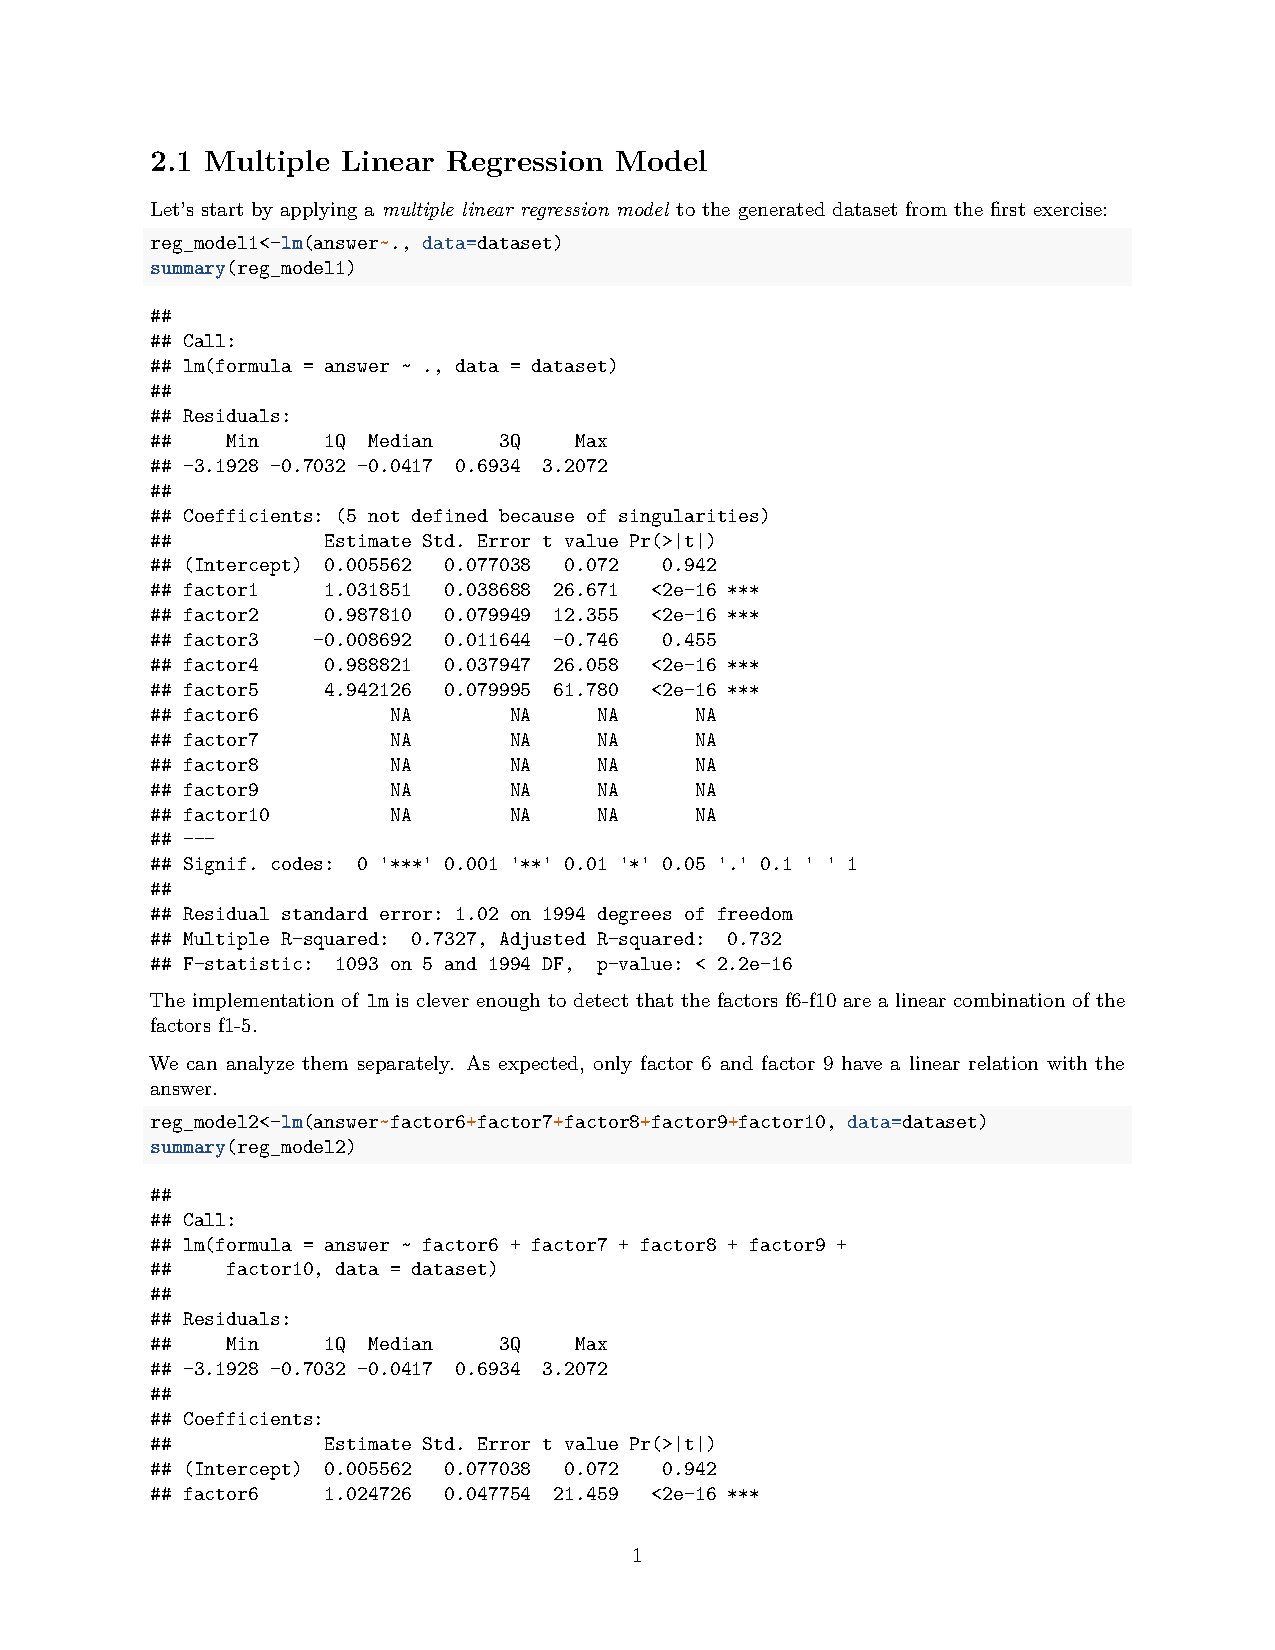
\includepdf[pages={1-}]{../ex2/ex2-no-title-statement.pdf}

%%%%%%%%%%%%% Exercise 3

\section{Simulate New Data}

For this part, we will use the expression obtained from the \textit{LRM} in the previous section and the framework \textit{GPSS} to simulate the data. Here is an snippet \ref{listing:3} of the GPSS code used to generate the model data. The rest of the scripts can be found on the directory \code{ex3/}.

\bigbreak

\begin{lstlisting}[caption={GPSS script to simulate data}, captionpos=b]
; factor |   min     |   max     |
; -------|-----------|-----------|
; f1     | 0.000836  | 3.483189  |
; f2     | 0.0000648 | 0.9997571 |
; f4     | 0.00125   | 3.43439   |
; f5     | 0.0001625 | 0.9991915 |

; f1 -
; f2 -
; f4 -
; f5 -

; Answer = 0.005562 + 1.032*f_1 + 0.988*f_2 + 0.988*f_4 + 4.94*f_5

GENERATE 1
ADVANCE  (1.032 # 0.000836  + DUNIFORM(RN1, 0, 1)) ;Factor 1
ADVANCE  (0.988 # 0.0000648 + DUNIFORM(RN1, 0, 1)) ;Factor 2
ADVANCE  (0.988 # 0.00125   + DUNIFORM(RN1, 0, 1)) ;Factor 4
ADVANCE  (4.94  # 0.0001625 + DUNIFORM(RN1, 0, 1)) ;Factor 5
TERMINATE 1
\end{lstlisting}
\label{listing:3}

Apart from the previous code, I used included an script to do the replication for the experimental design.

\subsection{Validation of the simulation}

In order to validate we used some operational validation techniques:\\

\begin{itemize}
  \item \textbf{Black Box validation}: we compared the real system data with the simulated data to validate its accuracy. We used \textit{Student's t-test} to validate that the model produced from the \textit{LRM} is accurated with respect to the real system. Formaly, \textit{Student's t-test} null hypothesis is that there is no statistical difference between the mean of the given two population.

  \item \textbf{GPSS Traces}: we used the simulation traces to compare the results, and analyze if the logic of the events are coherent with the understanding the experts have of the system. \\
\end{itemize}

We used the following \textit{R} script \ref{listing:2} for the \textit{Black Box validation} by the \textit{Student's t-test}. The resulting $p-value = 0.08 \geq \alpha = 0.05$. So we can accept the null hypothesis that is that the populations have the same mean. Hence, our model is a good approximation of the reality.

\begin{listing}[ht]
  \inputminted[fontsize=\footnotesize]{r}{../ex3/validation.R}
  \caption{Validation script}
\label{listing:2}
\end{listing}

%%%%%%%%%%%%% Exercise 4

\section{Design of Experiment}

In this section we will use the previously generated model data and analyze the interaction of these records with the answer dependent variable. The code for this section can be found at \code{ex4/}.

For this part, I wrote another haskell script (see Appendix \ref{s:appendix}) to run the Yates algorithm on the output of the generated data.

The result of Yates can be found at \code{ex4/yates.txt}. The file contains 1024 interactions so it is time consuming to analyze by hand. I made a small script to get the most significant factors. As expected, the factors are consistent with the experiment results (see listing \ref{listing:2}).

\begin{listing}[ht]
  \inputminted[fontsize=\footnotesize]{r}{../ex4/yates_single_factor.txt}
  \caption{Single factors from \code{ex4/yates.txt}}
\label{listing:2}
\end{listing}

We finish our experimental design by analyzing the results of the factorial experiment. The main factors of our model are:

\begin{itemize}
  \item Factor 1
  \item Factor 2
  \item Factor 4
  \item Factor 5
  \item Combinations of the previous ones.
\end{itemize}

that are the ones that we used to generate our system answer. \textbf{So, we can conclude that our model is an accurate representation of the reality}.


%%%%%%%%%%%%%%%% Appendix %%%%%%%%%%%%%%%%%%%%%

\newpage
\section*{Appendix}\label{s:appendix}

\subsection*{Yates implementation in Haskell}%
\label{sub:Yates implementation in Haskell}

\inputminted{haskell}{../ex4/Main.hs}\label{listing:4}

\end{document}
